\documentclass[../main.tex]{subfiles}

\begin{document}

\section{Meson mixing en oscillaties}%
\label{sec:meson_mixing_en_oscillaties}

\subsection{2-state systemen}%
\label{sub:2_state_systemen}

Meson mixing is niets meer dan gewone kwantummechanica. Als 2 toestanden dezelfde kwantumtoestanden binnen de behoudswetten zullen deze 2 toestanden opmengen met elkaar, in essentie zijn dit dezelfde toestanden. Hebben we $A$ en $B$ als 2 zo een toestanden dan krijgen we
\begin{equation}
    \begin{aligned}
        \label{eq:opmenhing_2_toestanden}
        A & \leftrightarrow B \\
        \left| \phi\right>&=c_{a}\left|\phi_{a}\right>+c_{b}\left| \phi_{b} \right>\\
        |\phi|^{2} &=\left|c_{a}\right|^{2}+\left|c_{b}\right|^{2}
    \end{aligned}
\end{equation}
Hierbij is de uiteindelijke golffunctie van deze 2 deeltjes een opmenging van de 2. De waarschijnlijkheden voor het ene of andere deeltje kunnen afhangen van de tijd en zullen dus oscileren. Een opmerking hierbij is dat bijvoorbeeld een elektron niet in een positron zal kunnen oscileren vanwege het behoud van lading. Voor de oscilatie tussen het proton en neutron is dit iets ingewikkelder. Alle krachten behalve de zwakke interactie behouden de isospin en zullen dus niet in elkaar oscileren. Dit is niet het geval bij de zwakke interactie die deze deeltjes met veel plezier zal laten overgaan. Zo is het alleen mogelijk dat deeltje/antideeltjes in elkaar kunnen overgezet worden waarbij behoud van massa lettend op overlappende breedtes ook behouden moet worden. Daarboven moet de lading ook behouden worden en houden we enkel neutrale toestanden over zoals neutrale mesonen en neutrinos.

\subsection{Meson mixing}%
\label{sub:meson_mixing}

Met de restricties hierboven opgenoemd zijn er nog maar een aantal mogelijke meson opmenginen mogelijk. Deze zijn:
\begin{equation}
    \begin{aligned}
        \label{eq:mogelijke_meson_opmengingen}
        \begin{array}{ll}
            \left|K^{0}\right>=\left| d \bar{s}\right> & \left|\bar{K}^{0}\right>=\left| \bar{d} s\right> \\
            \left|D^{0}\right>=\left| c \bar{u}\right> & \left|\bar{D}^{0}\right>=\left| \bar{c} u\right> \\
            \left|B_{d}^{0}\right>=\left| d \bar{b}\right> & \left|\bar{B}_{d}^{0}\right>=\left| \bar{d} b\right> \\
            \left|B_{s}^{0}\right>=\left| s \bar{b}\right> & \left|\bar{B}_{s}^{0}\right>=\left| \bar{s} b\right>
        \end{array}
    \end{aligned}
\end{equation}
De onderindex $d$ of $s$ bij het $B$ meson wijst op het hebben van een $d$ of $s$ quark. De reden waarom $\pi^0=\left|u\bar{u}\right>$ hier niet bij zit is omdat dit dezelfde hetzelfde zijn bij uitwisseling. Historisch zagen we dat $\bar{K}^{0}$ en $K^{0}$ vervallen in 2 en 3 pionen wat zou zeggen dat de pariteit van dit meson zowel $\pm1$ is.
\begin{equation}
    \begin{aligned}
        \label{eq:kaon_pion_verval}
            \bar{K}^{0} / K^{0} & \rightarrow & 2 \pi & & P=C P=+1 \\
                                & \rightarrow & 3 \pi & & P=C P=-1
    \end{aligned}
\end{equation}
Deze oscillaties gebeuren door 2 zwakke wisselwerkingen, $K^{0} \leftrightarrow(2 / 3) \pi \leftrightarrow \bar{K}^{0}$. Dit is het oude beeld dat we hiervan hebben.

\subsection{Box diagrammen}%
\label{sub:box_diagrammen}

Vandaag de dag weten we dat deze kaonen bestaan uit elk 2 quarks die aan de hand van $W$ bosonen zullen uitwisselen.

\begin{figure}[h]
    \centering
    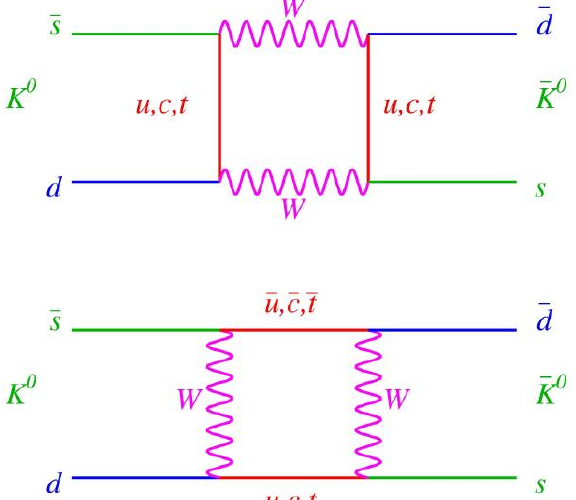
\includegraphics[width=0.4\linewidth]{meson_mixing_and_oscillations/box_diagrams.png}
    \caption{Box diagrammen van de kaon oscilaties}%
    \label{fig:meson_mixing_and_oscillations/box_diagrams}
\end{figure}

Zoals je kan zien is dit een 2de orde zwakke wisselwerkingen wat natuurlijk heel onwaarschijnlijk maar niet onmoglelijk is en de pariteit zal geschonden worden. Wat van groot belang is dat we intermediar naast de $W$ bosonen ook een een quark of antiquark zijn. We zijn hier dus met andere woorden gevoelig voor de koppeling tussen $d$ of $s$ en $u$, $c$ of $t$. Dit is iets waar we vandaag de dag nog veel onderzoek naar doen. Op dit moment gaan we er nog van uit dat de $CP$ pariteit behouden is.

\subsection{Mixen}%
\label{sub:mixen}

We gaan er hier van uit de $CP$ nog behouden is maar zien in dat $\bar{K}^{0}$ en $K^{0}$ niet de correcte eigentoestanden zijn omdat deze in elkaar worden omgezet.
\begin{equation}
    \begin{aligned}
        \label{eq:cp_anti_kaon}
        C P\left|K^{0}\right>=\left| \bar{K}^{0}\right>\quad C P\left|\bar{K}^{0}\right>=\left| K^{0}\right>
    \end{aligned}
\end{equation}
Het vervallen naar 2 verschillende hoeveelheden pionen is nu geen probleem meer omdat dit niet eens eigentoestanden zijn van $CP$ maar wel van $P$. Om correct te vervallen naar 2 of 3 pionen die $CP$ pariteit volgen moeten we ook voor de kaonen $CP$ eigentoestanden bepalen.
\begin{equation}
    \begin{aligned}
        \label{eq:kaon_cp_eigentoestanden}
        \left| K_{1}^{0}\right>&=\frac{1}{\sqrt{2}}\left[\left|K^{0}\right>+\left| \bar{K}^{0}\right>\right] & & C P=+1 \\
        \left| K_{2}^{0}\right>&=\frac{1}{\sqrt{2}}\left[\left|K^{0}\right>-\left| \bar{K}^{0}\right>\right] & & C P=-1
    \end{aligned}
\end{equation}
Dit kan ook nog herschreven worden tot
\begin{equation}
    \begin{aligned}
        \label{eq:kaon_cp_eig_mat}
        \left(\begin{array}{c}
            \left| K_{1}^{0}\right> \\
            \left| K_{2}^{0}\right>
            \end{array}\right)=\left(\begin{array}{cc}
                \cos \theta & \sin \theta \\
                -\sin \theta & \cos \theta
            \end{array}\right)\left(\begin{array}{c}
            \left| \bar{K}^{0}\right> \\
            \left| K^{0}\right>
        \end{array}\right)\\
        \left(\begin{array}{c}
            \left| m_{1}\right> \\
            \left| m_{2}\right>
            \end{array}\right)=\left(\begin{array}{cc}
                \cos \theta & \sin \theta \\
                -\sin \theta & \cos \theta
            \end{array}\right)\left(\begin{array}{c}
            \left| s_{1}\right> \\
            \left| s_{2}\right>
        \end{array}\right)
    \end{aligned}
\end{equation}
Dit zal dus een relatie geven tussen de massa eigentoestanden die vrij kunnen rond bewegen en de symmetrie eigentoestanden met definiete strangeness. In dit geval is de $\theta=45^\circ$. In essentie zijn de $s$ eigentoestanden van de sterke wisselwerking die de kaonen maakt en de $m$ eigentoestanden van de zwakke wisselwerking die zullen vervallen naar de pionen.\\
Hierbij moet de $CPT$ nog steeds behouden zijn wat wil zeggen dat $m(part) = m(\bar{part})$ of de $m(K^0) = m(\bar{K}^0)$ moet zijn. Maar de $\left|\bar{K}_{1}^{0}\right>\neq\left| K_{2}^{0}\right>$ en dat de massas niet perse gelijk moeten zijn aan elkaar. De massa van het kaon zal dus afhangen van hoe we er naar kijken, met de zwakke of sterke wisselwerking.

\subsection{Oscillaties}%
\label{sub:oscillaties}

Tijdens de oscillatie zal de massa eigentoestand propageren: $m_{i}(t)=m_{i}(0) e^{-i\left(m_{i}-i \frac{\Gamma_{i}}{2}\right) t}$. Hierbij wordt verondersteld dat de kaonen stil staan en een massa hebben. De 2de term in de exponent geeft de vervalsnelheid van de massatoestanden naar pionen terug.\\
Bekijken we nu het voorbeeld waar op tijdstip $t=0$ een pure $s_2$ toestand wordt waargenomen. Dit komt overeen met $s_{1}(0)=0, s_{2}(0)=1$. Indien we deze toestanden nu stabiel beschouwen hebben we $\Gamma_i = 0$ en krijgen we voor de massa toestanden:
\begin{equation}
    \begin{aligned}
        \label{eq:voorbeeld_osc_stable_massa}
        s_{1}(0)=m_{1}(0) \cos \theta-m_{2}(0) \sin \theta=0 \\
        s_{2}(0)=m_{1}(0) \sin \theta+m_{2}(0) \cos \theta=1
    \end{aligned}
\end{equation}
Om aan dit stelsel te voldoen moet $m_1(0) = \sin\theta$ en $m_2(0) = \cos\theta$ zijn. Vullen we de tijd propagatie door dan krijgen we 
\begin{equation}
    \begin{aligned}
        \label{eq:voorbeeld_osc_stable_massa_tijd_prop_1}
        s_{1}(t) &=m_{1}(t) \cos \theta-m_{2}(t) \sin \theta \\
                 &=\sin \theta \cos \theta\left[e^{-i m_{1} t}-e^{-i m_{2} t}\right] \\
                 &=\frac{\sin (2 \theta)}{2} e^{-\frac{i\left(m_{1}+m_{2}\right) t}{2}}\left[e^{-\frac{i\left(m_{1}-m_{2}\right) t}{2}}-e^{-\frac{i\left(m_{2}-m_{1}\right) t}{2}}\right]
    \end{aligned}
\end{equation}
De reden voor het herschrijven naar de uitgebreide vorm is omdat we nu mooie oscillatietermen krijgen die we kunnen herschrijven naar sinussen ($\sin (\theta) = \frac{1}{2 i}\left(e^{+i \theta}-e^{-i \theta}\right)$).
\begin{equation}
    \begin{aligned}
        \label{eq:voorbeeld_osc_stable_massa_tijd_prop_2}
        s_{1}(t)=\frac{\sin (2 \theta)}{2}(2 i) \sin \left(\frac{\Delta m \cdot t}{2}\right) e^{-\frac{i\left(m_{1}+m_{2}\right) t}{2}}
    \end{aligned}
\end{equation}
Zo kan je zien dat er een oscilatie volgens de tijd zal komen inkruipen in deze uitwerking. De waarschijnlijkheid om $s_1$ te vinden wordt gegeven door:
\begin{equation}
    \begin{aligned}
        \label{eq:voorbeeld_osc_stable_massa_prob_1}
        P\left(s_{1}\right)=\left|s_{1}(t)\right|^{2}=\sin ^{2}(2 \theta) \sin ^{2}\left(\frac{\Delta m \cdot t}{2}\right)
    \end{aligned}
\end{equation}
Door het kwadrateren van $s_1$ zal de exponentiële factor weg vallen. Belangrijk om te zien is dat de amplitude bepaald wordt door $\theta$ met een maximale waarde bij $\sin^2(2\theta)=1 \rightarrow \theta=45^\circ$ en deat de periode bepaald wordt door $\Delta m$.
\begin{equation}
    \begin{aligned}
        \label{eq:voorbeeld_osc_stable_massa_prob_2}
        P\left(s_{2}\right)=1-\left|s_{1}(t)\right|^{2}=1-\sin ^{2}(2 \theta) \sin ^{2}\left(\frac{\Delta m \cdot t}{2}\right)
    \end{aligned}
\end{equation}

\subsection{$K^0$-systeem}%
\label{sub:_k_0_systeem}

Nu we weten hoe de waarschijnlijkheid er uit ziet voor deeltjes die niet vervallen kunnen we het onszelf iets moeilijker maken door de kaonen ook te laten vervallen. Kijken we naar de massatoestanden van het kaon die zo goed als dezelfde massa hebben.\\
\begin{minipage}[c]{0.5\textwidth}
    \begin{center}
        $\left| K_1 \right> \rightarrow 2\pi$
    \end{center}
    \begin{itemize}
        \item Omdat deze maar vervalt in 2 pionen is er nog veel faseruimte over (een factor $p^2 dp$ aanwezig).
        \item Wordt waargenomen als $\left| K_S^0 \right>$
        \item Omdat deze veel faseruimte over heeft zal hij ook snel vervallen.
            \begin{equation}
                \begin{aligned}
                    \label{eq:verval_ks}
                    \tau_{S}&=(8.954 \pm 0.004) \cdot 10^{-11} \text{s}\\
                    \Gamma_S &= 7.4\mu\text{eV}\\
                    c\tau_S &= 2.6844\text{cm}
                \end{aligned}
            \end{equation}
    \end{itemize}
\end{minipage}\noindent
\begin{minipage}[c]{0.5\textwidth}
    \begin{center}
        $\left| K_2 \right> \rightarrow 3\pi$
    \end{center}
    \begin{itemize}
        \item Deze heeft niet veel faseruimte over
        \item Wordt waargenomen als $\left| K_L^0 \right>$
        \item Omdat deze weinig faseruimte over heeft zal hij ook langer leven.
            \begin{equation}
                \begin{aligned}
                    \label{eq:verval_ks}
                    \tau_{L}&=(5.116 \pm 0.021) \cdot 10^{-8} \text{s}\\
                    \Gamma_L &= 0.013\mu\text{eV}\\
                    c\tau_L &= 15.34\text{m}
                \end{aligned}
            \end{equation}
    \end{itemize}
\end{minipage}
Met deze informatie bekijken we nu de het voorbeeld waar bij $t=0$ het systeem zich in een pure $\left| K^0 \right>$ toestand bestaat. Dit wilt dus zeggen dat $K^0(0) = 1$ en $\bar{K}^0 = 0$ of $K_1(0)=K_2(0)= \frac{1}{\sqrt{2}} $. Propageren we deze toestanden nu door de tijd dan krijgen we op tijdstip $t$:
\begin{equation}
    \begin{aligned}
        \label{eq:voorbeeld_kaon_osc_tijd_prop_1}
        K^{0}(t) &=\frac{1}{\sqrt{2}}\left(K_{1}(t)+K_{2}(t)\right) \\
        \bar{K}^{0}(t) &=\frac{1}{\sqrt{2}}\left(K_{1}(t)-K_{2}(t)\right)
    \end{aligned}
\end{equation}
Vullen we hier de propagatie van de massatermen uit de vorige sectie in dan krijgen we:
\begin{equation}
    \begin{aligned}
        \label{eq:voorbeeld_kaon_osc_tijd_prop_2}
        K^{0}(t) &=\frac{1}{2}\left(e^{-i m_{1} t-\frac{\Gamma_{1}}{2} t}+e^{-i m_{2} t-\frac{\Gamma_{2}}{2} t}\right) \\
        \bar{K}^{0}(t) &=\frac{1}{2}\left(e^{-i m_{1} t-\frac{\Gamma_{1}}{2} t}-e^{-i m_{2} t-\frac{\Gamma_{2}}{2} t}\right)
    \end{aligned}
\end{equation}
Het verschil met vorige sectie \ref{sub:oscillaties} is nu dat de vervaltermen in de exponenten aanwezig zijn. Dit zal de berekening van de de probabiliteiten wel iets moeilijker maken. De waarschijnlijkheid dat we overgaan van een $K^0$ naar een $\bar{K}^0$ kan als volgt uitgewerkt worden.
\begin{equation}
    \begin{aligned}
        \label{eq:voorbeeld_kaon_osc_tijd_prop_3}
        P\left(K^{0} \rightarrow \bar{K}^{0}\right) &=\left|\bar{K}^{0}(t) \bar{K}^{0 *}(t)\right| \\
                                                    &=\frac{1}{4}\left(e^{-\Gamma_{1} t}+e^{-\Gamma_{2} t}-e^{+i \Delta m t} e^{-\Gamma t}-e^{-i \Delta m t} e^{-\Gamma t}\right) \\
                                                    &=\frac{1}{4}\left(e^{-\Gamma_{1} t}+e^{-\Gamma_{2} t}-2 \cos (\Delta m t) e^{-\Gamma t}\right)
    \end{aligned}
\end{equation}
Hierbij is $\Gamma = \frac{\Gamma_1 \Gamma_2}{2}$. Om van $K_0$ naar $K_0$ is nu makkelijk te vinden.
\begin{equation}
    \begin{aligned}
        \label{eq:voorbeeld_kaon_osc_tijd_prop_4}
        P\left(K^{0} \rightarrow K^{0}\right) &= 1-P\left(K^{0} \rightarrow \bar{K}^{0}\right)\\
                                              &=\frac{1}{4}\left(e^{-\Gamma_{1} t}+e^{-\Gamma_{2} t}+2 \cos (\Delta m t) e^{-\Gamma t}\right)
    \end{aligned}
\end{equation}
De waarschijnlijkheid dat er nog iets over is in het kaon systeem na tijd $t$ is
\begin{equation}
    \begin{aligned}
        \label{eq:voorbeeld_kaon_osc_tijd_prop_5}
        P\left(K^{0} \rightarrow \bar{K}^{0}\right)+P\left(K^{0} \rightarrow K^{0}\right)=\frac{1}{2}\left(e^{-\Gamma_{1} t}+e^{-\Gamma_{2} t}\right)
    \end{aligned}
\end{equation}
In figuur \ref{fig:meson_mixing_and_oscillations/kaon_osc_tijd_plot} worden een aantal waarschijnlijkheden geplot in de functie van de tijd onder bepaalde condities.

\begin{figure}[h]
    \centering
    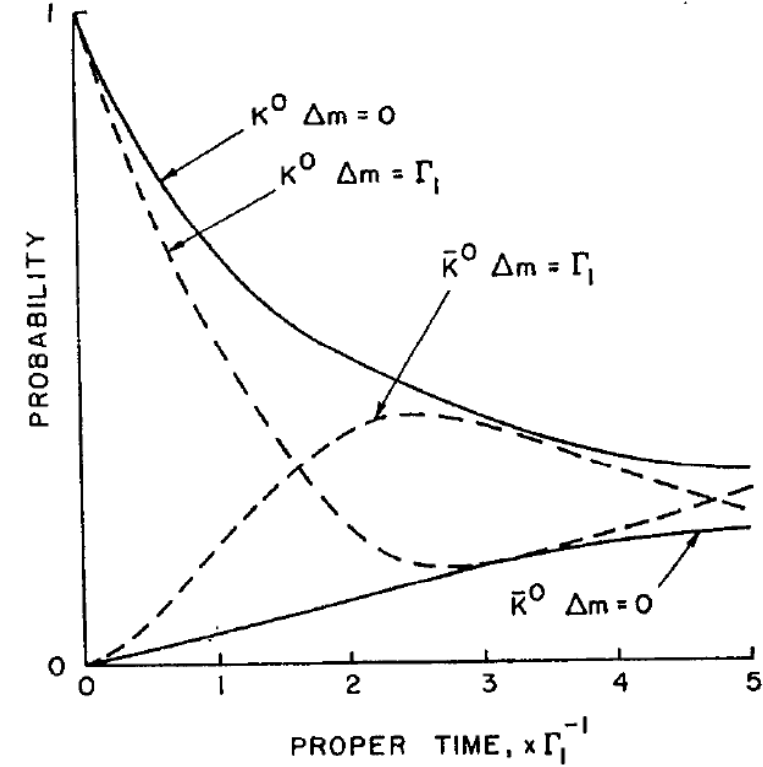
\includegraphics[width=0.5\linewidth]{meson_mixing_and_oscillations/kaon_osc_tijd_plot.png}
    \caption{Plot van kaon waarschijnlijkheden tijdens oscilaties}%
    \label{fig:meson_mixing_and_oscillations/kaon_osc_tijd_plot}
\end{figure}

Ten eerste als we kijken naar het geval dat de massa van de kaonen gelijk zijn ($\Delta m = 0$) valt de $\cos(\Delta m t)$ weg uit de vergelijkingen en kwasi exponentieel verval voor $K_0$. In het begin van de oscillaties wordt het verval geleid door $\Gamma_1$ en later door $\Gamma_2$. Indien $\Delta m$ verschillend van 0 is dan zal het meest waarschijnlijke deeltje afwisselen in de tijd waarbij de amplitude tussen de probabiliteiten afneemt in de tijd.\\
De belangrijkste puntjes dat we hier moeten onthouden zijn:
\begin{itemize}
    \item De kaonen oscileren enkel als $\Delta m \neq 0$.
    \item Het exponentiële verval wordt gedomineerd door de kortste levensduur. Voor het Kaon systeem is dit $K_S$.
\end{itemize}

\subsection{Experiment}%
\label{sub:experiment}

Hoe is het nu mogelijk om een onderscheid te maken tussen $K^0$ en $\bar{K}^0$?\\
Kijken we naar deze kaonen met de sterke interactie dan zien we het volgende:
\begin{equation}
    \begin{aligned}
        \label{eq:kaon_sterke_int}
        \bar{K}^{0}+p &\rightarrow & \pi^{+}+\Lambda \\
        \bar{d} s+u u d & &\rightarrow u \bar{d}+u d s \\
        K^{0}+p & &\centernot\rightarrow \pi^{+}+\Lambda \\
        d \bar{s}+u u d & &\centernot\rightarrow u \bar{d}+u d s
    \end{aligned}
\end{equation}
Als we kijken naar de quarks van de kaonen en het proton zal het voor $K^0$ niet mogelijk zal zijn om $\bar{s}$ door te geven om een $\Lambda$ te maken. $K^0$ zal dus zo goed als niet interageren met het proton.\\
Aan de hand van de zwakke interactie is het ook mogelijk om het verschil tussen de kaonen aan te voelen. Het zal altijd de $s$ quark of antiquark zijn die via een $W^\pm$ boson zal vervallen naar een $u$ quark of antiquark.

\begin{figure}[h]
    \centering
    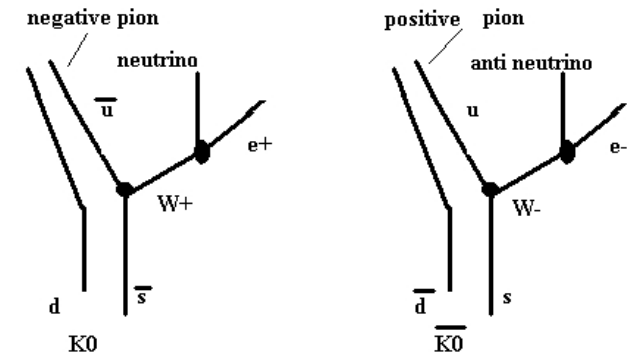
\includegraphics[width=0.4\linewidth]{meson_mixing_and_oscillations/kaon_zwak_verval.png}
    \caption{Feynman diagrammen van het zwak verval van kaonen}%
    \label{fig:meson_mixing_and_oscillations/kaon_zwak_verval}
\end{figure}

Hierdoor krijgen we verschillende einddeeltjes die in experimenten makkelijk uit elkaar te houden zijn.
\begin{equation}
    \begin{aligned}
        \label{eq:kaon_zwak_verval}
        \bar{K}^{0} &\rightarrow \pi^{+}+e^{-}+\bar{\nu}_{e} \\
        K^{0} &\rightarrow \pi^{-}+e^{+}+\nu_{e}
    \end{aligned}
\end{equation}
Het verval van het $W$ boson kan natuurlijk ook hadronisch gebeuren en krijgen we 2 keer dezelfde uiteindelijke toestand $\pi^+\pi^-$. Bij het verval naar leptonen hebben we niet een bepaalde $CP$ net zoals bij de kaon toestanden.\\
Wat gebeurt er nu juist. We maken aan de hand van de sterke interactie een zuivere $\left|K^0\right>=\left|\bar{d}s\right>$ toestand aan. Het vervallen van deze toestand is enkel mogelijk via de zwakke interactie op een semi leptonische manier (veglijking (\ref{eq:kaon_zwak_verval})) of op een hadronische manier. Hierbij wordt er ofwel vervallen via de $K^0$ en $\bar{K}^0$ componenten of van de $K_1$ en $K_2$ componenten.\\
Het is dus mogelijk aan de hand van assymetrie van de lading van de uitkomende leptonen te weten wat de ratio aan $K^0/\bar{K}^0$ te taggen.
\begin{equation}
    \begin{aligned}
        \label{eq:lepton_lading_assymetrie}
        A=\frac{N_{+}-N_{-}}{N_{+}+N_{-}}
    \end{aligned}
\end{equation}
Deze $A$ zal tussen -1 en 1 varieren met 1 die overeen komt met $t=0$ en 0 als er even veel $K^0$ en $\bar{K}^0$ aanwezig zijn. Deze oscillaties zijn mooi gemeten in experimenten.

\begin{figure}[h]
    \centering
    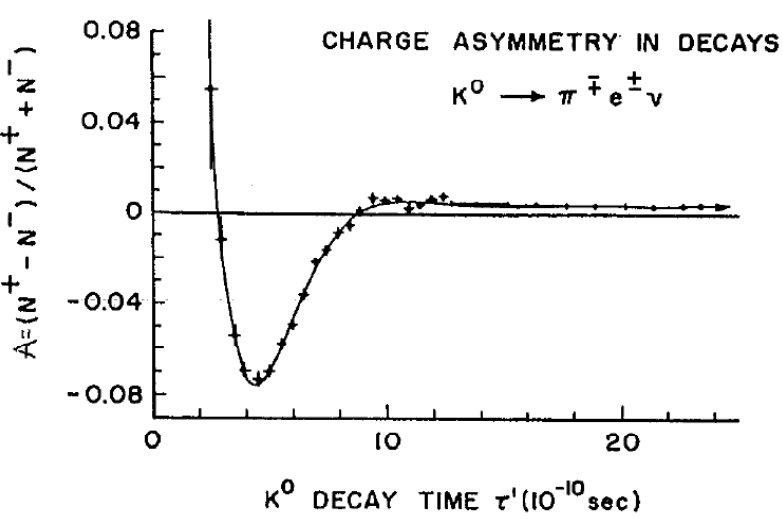
\includegraphics[width=0.5\linewidth]{meson_mixing_and_oscillations/kaon_osc_verval.png}
    \caption{Assymetrie onderzoek van de kaon oscilaties}%
    \label{fig:meson_mixing_and_oscillations/kaon_osc_verval}
\end{figure}

Dit gaat over heel kleine tijden. met een sterk gedempte oscilatie. Uit deze demping kunnen we het massaverschil bepalen $\Delta m=(0.5293 \pm 0.0009) \times 10^{-10} \text{s}^{-1} = (3.484 \pm 0.006) \times 10^{-12} \text{MeV}$. De reden waarom dit niet volledig naar 0 gaat is door $CP$ schending waar we later op verder gaan.

\subsection{Regeneratie}%
\label{sub:regeneratie}

Vertrekken we met een bundel kaonen $K^0$ of $\bar{K}^0$. Die zullen direct beginnen vervallen in pionen waarbij de $K_S$ met een weglengte van 3cm na 10cm allemaal vervallen zijn naar 2 pionen. We hebben dus alleen nog maar $K_L$ over. Plaatsen we in deze bundel nu een bulk materiaal. Kaonen zijn ongeladen deeltjes dus zullen ze makkelijk door het materiaal bewegen. In het materiaal zullen de kaonen sterk interageren met de nucleonen (nucleaire reacties). Na de botsing kunnen we terug spreken over $K^0$ en $\bar{K}^0$ omdat deze sterke wisselwerking ondergaan zijn. Er zullen naast $K_L$ ook terug $K_S$ aanwezig zijn. We hebben ze als het ware geregenereerd. Dit gaat als volgt:
\begin{equation}
    \begin{aligned}
        \label{eq:ks_regen}
        K_{L}=K_{2}&=\frac{1}{\sqrt{2}}\left(K^{0}-\bar{K}^{0}\right)\\
        \rightarrow \frac{1}{\sqrt{2}}\left(f K^{0}-\bar{f} \bar{K}^{0}\right)&=\frac{1}{2}\left(f\left(K_{S}+K_{L}\right)-\bar{f}\left(K_{S}-K_{L}\right)\right) \\
                                                                              &=\frac{1}{2}\left((f-\bar{f}) K_{S}+(f+\bar{f}) K_{L}\right)
    \end{aligned}
\end{equation}
In het geval dat $f\neq \bar{f}$ zien we dat $K_S$ zal geregenereerd worden. Kijken we alleen al naar de interactie van de kaonen met het proton (vergelijking (\ref{eq:kaon_sterke_int})) vergelijken zien we al direct dat $f$ groter zal zijn dan $\bar{f}$.

\subsection{Tijd afhankelijkheid}%
\label{sub:tijd_afhankelijkheid}

We hebben al gezien dat de tijd afhankelijkheid bepaald wordt door $\Delta m$. Integreren we dit over de tijd kunnen we zien wat de waarschijnlijkheid was om van $K^0$ naar $\bar{K}^0$ te gaan in vergelijking tot de totale oscillaties.
\begin{equation}
    \begin{aligned}
        \label{eq:kaon_osc_tijd_int}
        \chi=\frac{\int_{0}^{\infty} P\left(K^{0} \rightarrow \bar{K}^{0}\right) d t}{\int_{0}^{\infty}\left(P\left(K^{0} \rightarrow \bar{K}^{0}\right)+P\left(K^{0} \rightarrow K^{0}\right)\right) d t}=\frac{1}{2} \frac{x^{2}+y^{2}}{1+x^{2}}
    \end{aligned}
\end{equation}
met $x= \frac{\Delta m}{\Gamma}$ en $y= \frac{\Delta \Gamma}{2\Gamma} = \frac{\Gamma_L-\Gamma_S}{\Gamma_L + \Gamma_S}$. Hierbij zal $0\leq \chi \leq 0.5$ variëren. {\color{blue} Ryckbosch zegt dat het een goed idee is om deze integralen eens uit te rekenen maar zegt letterlijk dat dit geen examen leerstof is.} Deze verlijking zal iets zeggen over de opmenging. De $x$ zegt ons dat er enkel opmenging zal zijn als $\Delta m$ en $\Gamma$ van dezelfde orde moeten zijn.

\subsection{Kaon systeem resultaten}%
\label{sub:kaon_systeem_resultaten}

We zitten hier naar een effect te kijken van $\Delta m_K = (3.483 \pm 0.006) \times 10^{-6} \text{eV}$ tegenover de massa $m_K = 450$MeV. Dit betekent dat we kijken naar een effect $\sim O(10^{-15}$ kleiner dan de zijn massa nog steeds mooi zichtbaar is. De verval breedte van dit systeem komt overeen met $\Gamma=\frac{\Gamma_{S}+\Gamma_{L}}{2} \approx \frac{\Gamma_{S}}{2}=3.7 \times 10^{-6} \text{eV}$. Hier is het duidelijk dat $x$ ongeveer 1 zal zijn en de oscillatie zal doorgaan.
\begin{equation}
    \begin{aligned}
        \label{eq:kaon_osc_exp_results}
        x_{K} &=0.94 \\
        y_{K} &=0.998 \\
        \chi_{K} &=0.499
    \end{aligned}
\end{equation}
$x$ vertelt ons hoeveel oscillaties we krijgen per levensduur wat in dit geval dus 1 is.

\subsection{$B$-meson systeem}%
\label{sub:_b_meson_systeem}



\end{document}
